\documentclass[journal,10pt]{IEEEtran}
\IEEEoverridecommandlockouts

% --- Language and encoding ---
\usepackage[utf8]{inputenc}
\usepackage[T1]{fontenc}
\usepackage[english]{babel}

% --- Centered figure and table captions ---
\usepackage[justification=centering]{caption}

% --- Arabic numbering ---
\renewcommand{\thetable}{\arabic{table}}
\renewcommand{\thefigure}{\arabic{figure}}
\renewcommand{\thesection}{\arabic{section}}
\renewcommand{\thesubsection}{\thesection.\arabic{subsection}}
\renewcommand{\thesubsubsection}{\thesubsection.\arabic{subsubsection}}

% --- Essential packages ---
\usepackage{cite}
\usepackage{amsmath,amssymb,amsfonts}
\usepackage{graphicx}
\usepackage{textcomp}
\usepackage{xcolor}
\usepackage{booktabs}
\usepackage{array}
\usepackage{tabularx}
\usepackage[hidelinks]{hyperref}
\usepackage{xurl}

% --- TikZ and PGFPlots ---
\usepackage{pgfplots}
\pgfplotsset{compat=1.18}
\usepackage{tikz}
\usetikzlibrary{positioning,shapes.geometric,arrows.meta,fit,backgrounds}

\bibliographystyle{IEEEtran}
\def\IEEEbibitemsep{0pt plus .5pt}

\begin{document}

\title{V\'IA VIVA: An Edge-AI Vehicle-Mounted System for Detecting, Mapping and Predicting Road Hazards in Tunja, Colombia}

\author{Andr\'es Santiago C\'ardenas Gonz\'alez, Juan Felipe Garc\'ia Carvajal, Juan Diego Anzola Duarte, and Dany Alexander Cipamocha Ria\~no\\[0.3em]
\footnotesize andres.cardenasg@usantoto.edu.co \quad juan.garciac@usantoto.edu.co \quad juan.anzola@usantoto.edu.co \quad dany.cipamocha@usantoto.edu.co\\[0.15em]
\small Ingenier\'ia de Datos e Inteligencia Artificial --- Second semester\\
\small Universidad Santo Tom\'as, Seccional Tunja, Tunja, Colombia%
\thanks{Integrative Project 2026-2. Courses: Computer Architecture, Data Acquisition and Processing Systems (SADP), and Data Structures. Thematic line: Mobility.}}

\markboth{Universidad Santo Tom\'as, Seccional Tunja --- Integrative Project Proposal, 2026-2}%
{C\'ardenas \MakeLowercase{\textit{et al.}}: V\'IA VIVA --- Edge-AI Road Hazard Monitoring and Prediction}

\maketitle

\begin{abstract}
Road damage and unreported obstacles raise accident risk and vehicle costs in Tunja, Colombia, yet municipal road inspection still relies on manual field surveys. The city's new fixed traffic-enforcement cameras address driver violations, not the condition of the road itself. This proposal presents V\'IA VIVA, a low-cost system that combines vehicle-mounted edge-AI nodes, citizen reports and a georeferenced predictive model to build a live risk map of road hazards. The node pairs an ESP32-S3 microcontroller with an accelerometer, an inertial unit, a laser time-of-flight range sensor and a GPS receiver; a quantized (int8) classifier running on the node labels potholes, speed bumps and severe impacts and measures road roughness, and an ESP32-CAM captures anonymized photographic evidence only when an event occurs. A predictive model then estimates, for every street segment, the probability of hazards that have not yet been reported. Fleet-mounted nodes cover main roads, while a citizen-reporting module (chat bot or web form, with an SMS fallback for rural areas) covers neighborhoods, side streets and rural roads. An extract-transform-load (ETL) pipeline merges node events, citizen reports, web-scraped public sources and the OpenStreetMap street graph, and a dashboard ranks inspections and repairs for the authorities. The proposal specifies the acquisition chain, the computer-architecture design (bus selection, DMA double buffering, dual-core task split), the data structures, a set of measurable experiments, a four-week plan and a bill of materials of about 342\,000 COP for one prototype node.
\end{abstract}

\begin{IEEEkeywords}
Edge AI, TinyML, pothole detection, predictive maintenance, geospatial risk map, ESP32-S3, crowdsensing, ETL.
\end{IEEEkeywords}

% =========================================================================
\section{Introduction}
\IEEEPARstart{T}{he} condition of urban and rural roads directly affects safety, travel time and vehicle maintenance costs. In Tunja, the capital of the department of Boyac\'a, road damage is assessed through manual inspection: internship reports from the Universidad Santo Tom\'as civil engineering program at the municipal Infrastructure Secretariat describe field forms and on-foot surveys of pavement pathologies \cite{caballero2022practica}. Manual surveys are slow, infrequent and hard to scale to the rural road network that the departmental government (Gobernaci\'on de Boyac\'a) must also maintain.

Since March 2026, Tunja operates fixed photo-enforcement cameras on its main avenues to detect speeding, red-light violations and expired vehicle documents \cite{infobae2026tunja}. These systems are regulated by Law 1843 of 2017 \cite{ley1843} and are designed to sanction drivers. They do not report potholes, obstacles or stalled vehicles, and, being fixed, they cover only a handful of points.

This proposal describes V\'IA VIVA, a system that turns ordinary vehicles into mobile road sensors and lets citizens report hazards where the vehicles do not go. Detection happens on the device itself (edge AI), so only compact events---not continuous trajectories or raw video---leave the vehicle. The project is the integrative project of the second semester and combines three courses: Data Acquisition and Processing Systems (acquisition and signal processing), Computer Architecture (embedded hardware design and performance), and Data Structures (event fusion, prioritization and visualization). The declared thematic line is \textit{Mobility}.

% =========================================================================
\section{Justification}
Three gaps motivate the project. First, \emph{coverage}: manual inspection and fixed cameras observe only a small fraction of the road network at any time. Second, \emph{timeliness}: a pothole may remain unreported for weeks, and the authority has no objective way to rank repairs. Third, \emph{anticipation}: detection only finds damage where a vehicle passes, so the authority also needs to know where unreported damage is \emph{likely}. Public datasets such as RDD2022 cover six countries and not Colombia \cite{arya2022rdd}, so local data has value in itself.

Edge processing is justified by bandwidth and privacy: a raw 200~Hz inertial log (3.2~kB/s) shrinks to about 6.4~B/s when only 64-byte events are sent every 10~s on average, roughly 500 times less, and images are blurred on the node \cite{ley1581}.


% =========================================================================
\section{Objectives}
\subsection{General Objective}
To design and validate a prototype edge-AI system that detects, documents, maps and predicts road hazards in Tunja by fusing vehicle-mounted sensing, citizen reports and georeferenced data, giving the authorities a prioritized, evidence-based view of where to inspect and repair.

\subsection{Specific Objectives}
\begin{itemize}
\item \textbf{Data Acquisition and Processing Systems:} to build and characterize the acquisition chain (accelerometer, inertial unit, GPS and camera), choosing the sampling rate from measured spectra, synchronizing sensors in time, and extracting features for a lightweight classifier.
\item \textbf{Computer Architecture:} to design the node architecture (SPI, I\textsuperscript{2}C and UART buses, DMA double buffering, dual-core task split, two cooperating processors) and to measure latency, CPU load, memory usage and power consumption.
\item \textbf{Data Structures:} to implement the data structures that cluster events, map them onto the street graph, rank repairs and serve the dashboard, analyzing their computational complexity.
\item \textbf{ETL, scraping and prediction:} to build a pipeline that merges node, citizen and public web data per street segment, and a georeferenced model that predicts unreported hazards.
\end{itemize}

% =========================================================================
\section{Related Work}
Accelerometer-based road monitoring started with dedicated vehicle sensors \cite{eriksson2008pothole} and moved to smartphones \cite{mohan2008nericell,mednis2011pothole}. Crowd-sensing applications such as CRATER aggregate many users' measurements to estimate road quality \cite{kalim2016crater}. In computer vision, RDD2022 provides more than 47\,000 annotated road images with pothole and crack classes for training detectors \cite{arya2022rdd}. On the embedded side, integer-only quantization \cite{jacob2018quant} and TensorFlow Lite Micro \cite{david2021tflm} make it possible to run neural networks on microcontrollers, and TinyML benchmarking work highlights latency, memory and energy as the key metrics \cite{banbury2020tinyml}. Crowdsourced smartphone apps, however, depend on user participation and suffer from false positives. V\'IA VIVA combines these lines in a low-cost, locally deployable system: always-on fleet nodes, a citizen-reporting channel, confirmation of each hazard by independent sources, and a repair-prioritization layer for public authorities.

% =========================================================================
\section{Proposed System}
\subsection{Overview}
Fig.~\ref{fig:arch} shows the architecture. Vehicle nodes detect and document events; citizens report hazards from a chat bot or web form (with an SMS fallback in rural areas); and a server-side ETL pipeline merges all sources into a single map.

\begin{figure}[!t]
\centering
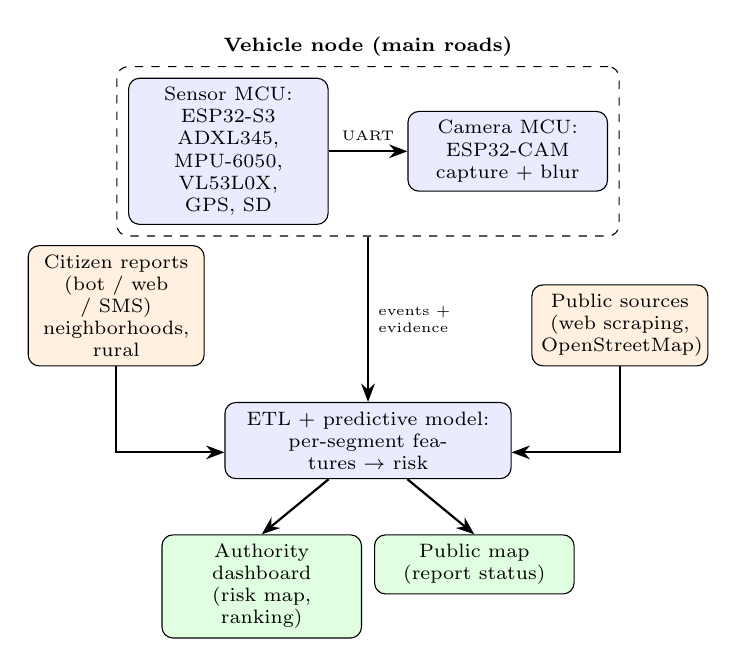
\begin{tikzpicture}[
  font=\scriptsize,
  blk/.style={draw, rounded corners, fill=blue!8, align=center, minimum height=0.8cm, text width=2.3cm},
  src/.style={draw, rounded corners, fill=orange!12, align=center, minimum height=0.8cm, text width=2.0cm},
  outb/.style={draw, rounded corners, fill=green!12, align=center, minimum height=0.75cm, text width=2.3cm},
  arr/.style={-{Stealth}, thick}
]
\node[blk] (sens) {Sensor MCU: ESP32-S3\\ADXL345, MPU-6050,\\VL53L0X, GPS, SD};
\node[blk, right=1.0cm of sens] (cam) {Camera MCU:\\ESP32-CAM\\capture + blur};
\draw[arr] (sens) -- node[above, font=\tiny]{UART} (cam);
\begin{scope}[on background layer]
\node[draw, dashed, rounded corners, fit=(sens)(cam), inner sep=4pt, label={[font=\scriptsize\bfseries]above:Vehicle node (main roads)}] (node) {};
\end{scope}
\node[blk, below=2.1cm of node.south, anchor=north, text width=3.4cm] (etl) {ETL + predictive model:\\per-segment features $\rightarrow$ risk};
\node[src, left=0.25cm of etl.north west, anchor=south east, yshift=0.45cm] (cit) {Citizen reports\\(bot / web / SMS)\\neighborhoods, rural};
\node[src, right=0.25cm of etl.north east, anchor=south west, yshift=0.45cm] (web) {Public sources\\(web scraping,\\OpenStreetMap)};
\draw[arr] (node.south) -- node[right, font=\tiny, align=left]{events +\\evidence} (etl.north);
\draw[arr] (cit.south) |- ([yshift=-0.15cm]etl.west);
\draw[arr] (web.south) |- ([yshift=-0.15cm]etl.east);
\node[outb, below=0.7cm of etl.south, anchor=north, xshift=-1.35cm] (dash) {Authority dashboard\\(risk map, ranking)};
\node[outb, below=0.7cm of etl.south, anchor=north, xshift=1.35cm] (map) {Public map\\(report status)};
\draw[arr] ([xshift=-0.5cm]etl.south) -- (dash.north);
\draw[arr] ([xshift=0.5cm]etl.south) -- (map.north);
\end{tikzpicture}
\caption{V\'IA VIVA architecture: vehicle nodes (blue), other data sources (orange) and outputs (green).}
\label{fig:arch}
\end{figure}

The coverage strategy is complementary: nodes mounted on fleet vehicles monitor the main roads they travel every day, while citizens cover neighborhoods, side streets and rural roads that the instrumented vehicles do not reach. Each hazard follows a life cycle---\textit{new}, \textit{confirmed}, \textit{under repair}, \textit{repaired}---and later passes of instrumented vehicles without impact help confirm the repair. Citizens see the status of their reports on the public map, which gives them a direct reason to keep reporting.

\subsection{Data Acquisition}
Each node carries an ADXL345 accelerometer (SPI, 32-sample FIFO with watermark interrupt \cite{adi_adxl345}) as the main sensor for potholes, bumps and impacts; an MPU-6050 (I\textsuperscript{2}C) that adds a gyroscope and serves as a bus baseline; a VL53L0X laser time-of-flight sensor (I\textsuperscript{2}C) pointed at the pavement to measure its profile and pothole depth (its range drops in strong sunlight, which will be tested); a NEO-6M GPS (UART) for position, speed and UTC time; an OV2640 camera for event evidence; a push button for ground-truth labels; and a microSD card for the raw log.



The sampling rate will be chosen from measurements rather than assumed: the first test drives will be recorded at a high rate, the power spectral density will be computed, and the lowest rate that keeps 95\,\% of the signal energy (with a margin above the Nyquist rate) will be selected. The working hypothesis is 200~Hz with an anti-aliasing cut-off near 80~Hz. Time synchronization is critical: at 30~km/h, a 300~ms timestamp error displaces an event by 2.5~m, and consecutive 1~Hz GPS fixes are 8.3~m apart (1.7~m at 5~Hz). Event positions will therefore be interpolated between fixes using the GPS UTC time. Because the node may be mounted in any orientation, gravity will be estimated while the vehicle is stopped and the signal rotated to the vertical axis.

\subsection{Computer Architecture of the Node}
The node uses an ESP32-S3 for sensing and inference (dual-core Xtensa LX7 at up to 240~MHz, 512~kB of SRAM, vector instructions for neural-network workloads \cite{espressif_s3}) and an ESP32-CAM for evidence. The sensor MCU runs acquisition and inference on one core and storage and communication on the other. When it detects an event, it requests a photograph from the camera MCU over UART, so the camera works only on demand.

The accelerometer FIFO raises an interrupt every 32 samples (every 160~ms at 200~Hz), and the samples are transferred by DMA into two alternating (ping-pong) buffers, so the CPU processes one buffer while the other fills. At this data rate the bus is not a bottleneck; the expected benefit of DMA is freeing the CPU for inference, logging and networking. The accelerometer and the microSD card use separate SPI buses to avoid contention. Table~\ref{tab:exp} lists the experiments that will quantify these design choices.

\begin{table}[!t]
\centering
\caption{Planned computer-architecture experiments.}
\label{tab:exp}
\footnotesize
\begin{tabularx}{\columnwidth}{@{}l>{\raggedright\arraybackslash}X>{\raggedright\arraybackslash}X@{}}
\toprule
\textbf{ID} & \textbf{Comparison} & \textbf{Metrics} \\
\midrule
E1 & Polling vs.\ per-sample interrupt vs.\ FIFO + DMA ping-pong & Sampling jitter, CPU load, lost samples, current \\
E2 & Model weights in flash (cached) vs.\ SRAM vs.\ PSRAM & Inference latency \\
E3 & float32 vs.\ int8, with and without vector kernels & Latency, RAM, flash, F1 \\
E4 & I\textsuperscript{2}C (MPU-6050) vs.\ SPI (ADXL345) & Read time, CPU occupancy \\
\bottomrule
\end{tabularx}
\end{table}

\subsection{Signal Processing and Edge AI}
The processing chain is: low-pass filtering, gravity removal, event-triggered windowing by energy or jerk, and speed-normalized features (peak, RMS, kurtosis, crest factor and band energies). Two classifiers will be compared: a decision tree or random forest exported to C, and a one-dimensional convolutional network quantized to int8 \cite{jacob2018quant} and deployed with TensorFlow Lite Micro \cite{david2021tflm}. The camera MCU performs simple detection and blurs license plates and faces before any image leaves the node; license-plate reading is explicitly out of scope.

\subsection{Data Structures}
On the node, a circular buffer holds signal windows and a queue holds events awaiting transmission (store-and-forward). On the server, a hash table indexed by geographic grid cells (geohash) clusters nearby events into a single hazard; this will be compared against brute-force search. The street network, obtained from OpenStreetMap \cite{boeing2017osmnx}, is stored as an adjacency-list graph; each hazard is assigned to a street segment, and breadth- or depth-first search groups hazards along the same corridor into a single work order. A binary heap ranks segments by risk and severity, and an ordered map (binary search tree) supports date-range queries; the dashboard is built in Java Swing.

\subsection{Citizen Reports, ETL and Web Scraping}
Citizens report hazards through a chat bot or web form that captures a photo and the exact GPS location. In rural areas without mobile data, a structured SMS (e.g., hazard type and place) received by an Android gateway phone serves as a fallback. The ETL pipeline extracts data from the nodes, the citizen channel and public web sources that allow automated access (official pages, RSS feeds, open data and weather information), then cleans, geocodes, matches each record to the street graph, removes duplicates and loads it into an SQLite database.

\subsection{Georeferenced Predictive Risk Model}
Detection only covers the streets the vehicle drives. To anticipate unreported hazards, each OpenStreetMap segment receives a feature vector: road class and surface, slope from a public elevation model, rainfall, known hazards nearby (node, citizen and municipal inventory), crash points, and the roughness index and pavement depth profile measured by the node. A logistic regression and a random forest, chosen for interpretability with small data, are trained on segments with known condition and validated with spatial cross-validation (whole neighborhoods held out). The output is a risk map and a ranked list of segments to inspect.

\section{Methodology}
The project follows the five phases defined in the integrative-project guidelines. Fig.~\ref{fig:phases} summarizes them, and the following subsections describe how each one will be executed.

\begin{figure}[!t]
\centering
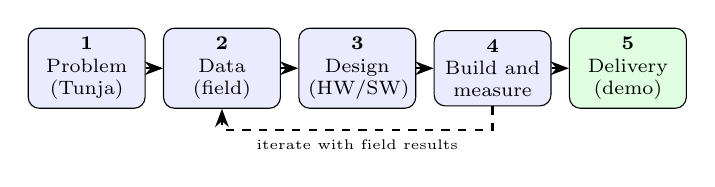
\begin{tikzpicture}[
  font=\scriptsize,
  ph/.style={draw, rounded corners, fill=blue!8, align=center, minimum height=0.9cm, text width=1.25cm},
  arr/.style={-{Stealth}, thick}
]
\node[ph] (p1) {\textbf{1}\\Problem\\(Tunja)};
\node[ph, right=0.22cm of p1] (p2) {\textbf{2}\\Data\\(field)};
\node[ph, right=0.22cm of p2] (p3) {\textbf{3}\\Design\\(HW/SW)};
\node[ph, right=0.22cm of p3] (p4) {\textbf{4}\\Build and\\measure};
\node[ph, right=0.22cm of p4, fill=green!12] (p5) {\textbf{5}\\Delivery\\(demo)};
\foreach \a/\b in {p1/p2,p2/p3,p3/p4,p4/p5} \draw[arr] (\a) -- (\b);
\draw[arr, dashed] (p4.south) -- ++(0,-0.3) -| node[pos=0.25, below, font=\tiny]{iterate with field results} (p2.south);
\end{tikzpicture}
\caption{Project phases; field results feed back into data collection.}
\label{fig:phases}
\end{figure}

\subsection{Phase 1: Problem Validation}
The problem will be validated with the stakeholders before freezing requirements. Formal requests were sent to Tunja's Infrastructure and Transit Secretariats (road inventory and crash points) and to the Gobernaci\'on de Boyac\'a, with an internal contact following them up.

\subsection{Phase 2: Field Data Collection}
A pilot zone of a few neighborhoods will be defined, with a route combining a main avenue, residential streets and an unpaved segment. Every pothole and speed bump on the route will be photographed and georeferenced by hand to build the ground truth. With the team's vehicle, the route will be driven repeatedly at 20, 30 and 40~km/h, in dry and, when possible, wet conditions. The driver only drives; a passenger presses the labeling button at each event. The first drives will be logged at a high sampling rate to measure the spectrum and fix the final rate. In parallel, the citizen channel will be piloted with classmates, who will report hazards in their own neighborhoods.

\subsection{Phases 3--4: Design, Implementation and Measurement}
Implementation proceeds by levels so that a working system exists early: Level~1 (sensor node, live map and ETL), Level~2 (camera evidence, citizen channel, scraping and repair ranking) and Level~3 (optional long-range radio). The classifiers will be validated with a \emph{leave-one-drive-out} scheme so that no drive appears in both training and test sets. The architecture experiments of Table~\ref{tab:exp} will be measured as follows: sampling jitter by timestamping each FIFO interrupt; CPU load from the real-time operating system's run-time statistics; and current with a USB power meter in each operating state (idle, acquisition, inference, storage and Wi-Fi). Finally, the risk model is validated in the field: the team drives to the ten highest-risk segments \emph{not yet reported} and to ten random segments, and compares how many contain hazards.

\subsection{Evaluation Metrics}
Table~\ref{tab:metrics} lists the metrics and the targets the team commits to. The targets are design goals; the final report will present measured values.

\begin{table}[!t]
\centering
\caption{Evaluation metrics and design targets.}
\label{tab:metrics}
\footnotesize
\begin{tabularx}{\columnwidth}{@{}>{\raggedright\arraybackslash}X l l@{}}
\toprule
\textbf{Metric} & \textbf{Course} & \textbf{Target} \\
\midrule
Pothole detection F1 score & SADP & $\geq 0.80$ \\
Event position error & SADP & $\leq 5$ m \\
False positives per km & SADP & $\leq 1$ \\
Inference latency per window & Arch. & $\leq 50$ ms \\
Lost samples under full load & Arch. & 0 \\
Node current (average) & Arch. & measured \\
RAM and flash usage & Arch. & measured \\
Duplicate reports merged & DS & $\geq 90$\,\% \\
Report-to-map delay & DS / ETL & $\leq 1$ min \\
Hit rate, top-10 risk vs.\ random & Pred. & higher \\
Risk-model AUC (spatial CV) & Pred. & $\geq 0.70$ \\
\bottomrule
\end{tabularx}
\end{table}

% =========================================================================
\section{Expected Results and Contributions}
The team expects to deliver: a characterized acquisition chain and the first labeled road-vibration dataset of Tunja (SADP); one working node with measured results of E1--E4 (Architecture); event clustering, graph matching and ranking with complexity analysis (Data Structures); and a field-validated risk map that shows the authority where to inspect and repair first.


% =========================================================================
\section{Budget and Schedule}
One prototype node will be built (Table~\ref{tab:budget}; quoted Oct.~2026); the team provides power, cables and mounts. Fig.~\ref{fig:gantt} shows the four-week schedule.

\begin{table}[!t]
\centering
\caption{Budget for one prototype node (COP).}
\label{tab:budget}
\footnotesize
\begin{tabularx}{\columnwidth}{@{}>{\raggedright\arraybackslash}Xr@{}}
\toprule
\textbf{Item group} & \textbf{Cost} \\
\midrule
Microcontrollers (ESP32-S3, ESP32-CAM) & 115\,000 \\
Sensors (2 ADXL345, MPU-6050, VL53L0X, GPS) & 98\,000 \\
Storage (microSD module and card) & 42\,000 \\
Enclosure, wiring and USB power meter & 51\,100 \\
Shipping and 5\,\% contingency & 36\,300 \\
\midrule
\textbf{Total} & \textbf{342\,400} \\
\bottomrule
\end{tabularx}
\end{table}

\begin{figure}[!t]
\centering
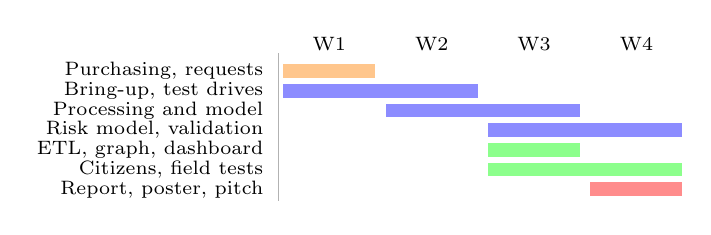
\begin{tikzpicture}[font=\scriptsize, x=1.3cm, y=0.25cm]
\foreach \w in {1,...,4} \node at (\w+1.9,0.9) {W\w};
\foreach \n/\s/\e/\c [count=\i] in {
  {Purchasing, requests}/1/1/orange,
  {Bring-up, test drives}/1/2/blue,
  Processing and model/2/3/blue,
  {Risk model, validation}/3/4/blue,
  {ETL, graph, dashboard}/3/3/green,
  {Citizens, field tests}/3/4/green,
  {Report, poster, pitch}/4/4/red}{
  \node[anchor=east] at (2.35,-\i+0.5) {\n};
  \fill[\c!45] (\s+1.45,-\i+0.15) rectangle (\e+2.35,-\i+0.85);
}
\draw[gray!60] (2.4,0.4) -- (2.4,-7.1);
\end{tikzpicture}
\caption{Four-week schedule, Oct.~19 -- Nov.~13, 2026.}
\label{fig:gantt}
\end{figure}

% =========================================================================
\section{Ethical and Legal Considerations}
\begin{itemize}
\item \textbf{Privacy by design.} Faces and license plates are personal data under Law 1581 of 2012 \cite{ley1581}; they are blurred on the node and the original image never leaves it. Nodes store events, not trajectories, and drivers give informed consent.
\item \textbf{No sanctions.} Fines are reserved for authorized equipment under Law 1843 of 2017 \cite{ley1843}; V\'IA VIVA provides evidence and statistics only.
\item \textbf{Responsible scraping and field safety.} Only sources whose terms and \texttt{robots.txt} allow it are scraped, and the driver never operates the system while driving.
\end{itemize}

% =========================================================================
\section{Conclusion}
V\'IA VIVA addresses a concrete need in Tunja: knowing where roads are damaged, where they are likely to be damaged, and which repairs matter most. It puts acquisition and computer architecture at the core, adds a georeferenced predictive layer, and fits four weeks and about 342\,000~COP.

\bibliography{referencias}

\end{document}
